\section{Experiments}



We compare 11 representative machine learning models, including GNN and GNN-RNN, on US county-level crop yields for corn and soybean. We evaluate performance on three metrics: RMSE, $R^2$, and correlation coefficient. Given a test year $t$, we use year $t-1$ for validation and all the prior years for training. For example, if the test year is 2019, we train on data from years 1981-2017 (inclusive), validate on 2018 crop yields, and test on 2019 crop yields.

\subsection{Dataset Details}

% NOte: see dataset_OLD.tex for more detailed text, if we need it in the future

Crop yield labels for corn and soybean are available from the USDA Crop Production Reports \cite{usda2013national} for numerous counties in the US. Not all counties report data in every year, but the coverage is still quite comprehensive. For example, for corn, all years between 1981 and 2003 have over 2,000 counties across $41$ states reporting data. We train and evaluate our model on all counties where yield data is available. (When computing the loss, we ignore counties that do not have yield labels for that year.)

We use a variety of climate, land surface, and soil quality variables as input features; these features are available for almost all counties in the contiguous 48 US states (3,107 counties in total\footnote{The only exception is Nantucket County, Massachusetts, where land surface model data is missing, since it is an offshore island. Also note that some counties have feature data but not label (yield) data. Only the GNN and GNN-RNN models can make use of these unlabeled county features.}). We draw 7 weather features from the PRISM climate mapping system \cite{daly2013prism}: precipitation, min/mean/max temperature, min/max vapor pressure deficit, and mean dewpoint temperature. These features are available at a $4 \times 4$ km grid for each day. 

We acquire 16 land surface features from the North American Land Data Assimilation System (NLDAS) \cite{xia2012continental}, which is a large-scale land surface model that closely simulates land surface parameters. These features include soil moisture content, moisture availability, and soil temperature (all at various soil depths), as well as observed weather variables such as wind speed and humidity. These variables are available at a $0.125 \times 0.125$ degree ($\sim 14$ km) spatial resolution, every hour. 

%We aggregate the hourly data to daily, and aggregate the grid to the county level in the same way as PRISM. 


% We acqui  gSSURGO dataset \cite{soil2019gridded} provides abundant survey-collected features regarding the soil composition and quality of an area. These gridded features are available at a 30-meter spatial resolution, and \emph{do not change over time}.

Soil quality features were acquired from the Gridded Soil Survey Geographic Database (gSSURGO) \cite{soil2019gridded}, at a $30 \times 30$ meter resolution. These features include available water capacity, bulk density, and electrical conductivity, pH, and organic matter.
% We used 20 features that are available at 6 different soil depth levels, as well as 6 ``extra'' features (such as crop productivity indices) that are not depth-dependent. 
Unlike the weather and land surface features, the gSSURGO soil quality features are fixed and \emph{do not change over time}. In addition to the raw features, we use the raw sand, silt, and clay percentages to compute the ``soil texture type'' of each pixel based on the Natural Resources Conservation Service Soil Survey's classification scheme \cite{soiltexture}, and then compute the fraction of each county occupied by each soil texture type. In total, we have a total of 20 gSSURGO variables that are depth-dependent (so there are values for 6 different soil depth levels), and 6 ``extra'' variables which are not depth-dependent (such as crop productivity indices). Finally, as in \cite{khaki2020cnn}, we use the average crop yield (over all counties) of the previous year as an additional input feature, to capture the increasing trend in crop yield over time. A full list of the features can be found in the Appendix.

%Again, we aggregate these features to the county level using the weighted-average technique, only considering pixels that are cropland/grassland/pasture.
% The North American Land Data Assimilation System (NLDAS) \cite{xia2012continental} is a large-scale land surface model that closely simulates land surface parameters. We collect 16 features from this dataset, including several ``forcing'' weather variables, as well as soil moisture, moisture availability, and soil temperature at multiple soil depths. These data are originally available at a $0.125 \times 0.125$ degree (roughly $14$ km) spatial resolution, and an hourly temporal resolution. We aggregate the hourly data to daily, and aggregate the grid to the county level in the same way as PRISM. 


All of these datasets were originally available as gridded raster data at a variety of spatial resolutions. We aggregated each feature to the county level by computing the weighted average of the variable over all grid cells that overlap with the county. Each grid cell is weighted by the percentage of the cell that lies inside the county, multiplied by the percentage of that grid cell which is cropland, pasture, or grassland; the land cover percentages are computed using the National Land Cover Database \cite{nlcd}. In addition, the time-dependent variables (weather and land surface) were aggregated from daily to weekly frequency to make the prediction task more tractable.

%Figure \ref{aggregating_to_county} shows an example of the process we use to aggregate gridded features to the county level.

% \begin{figure}[t]
% \centering
% \includegraphics[width=0.75\columnwidth]{figs/nldas.png}
% \includegraphics[width=0.75\columnwidth]{figs/nldas_SOILM_layer1_19810101_county.png}
% \caption{Example of aggregating features to county level. \\
% \textbf{(a)} raw raster of soil moisture from NLDAS. \\
% \textbf{(b)} Percentage cropland/grassland/pasture (used to compute grid cell weights).\\
% \textbf{(c)} the county-level values we generated. \textbf{make bigger, make size of figures consistent}}
% \label{aggregating_to_county}
% \end{figure}

\subsection{Compared Methods}

We consider two types of methods: \textbf{(a) single-year methods} that only use features from year $t$ to predict yield for the same year $t$, and \textbf{(b) 5-year methods} that use features from a 5-year series (years $\{t-4, t-3, \dots, t\}$) to predict yield for year $t$.

\textbf{Single-year methods.} We first consider methods that only use a single year of data to make predictions, to provide a fair comparison to the single-year GNN. For non-deep baseline methods, we select lasso, ridge regressor and gradient boosting regressor. For these methods, we flatten all the features from the entire year into a single feature vector, ignoring the temporal and soil-depth structure in the data.
Next, we tried three baseline deep learning architectures for $f_{wl}(\cdot)$: LSTM \cite{hochreiter1997long}, GRU \cite{chung2014empirical}, and 1-D CNN \cite{kalchbrenner2014convolutional}. All of these methods process the weekly time-series of weather and land surface data within the year. We compare these methods with our single-year GNN model (Eq. \ref{eq:gnn}), which incorporates geospatial context in making predictions.
 
\textbf{5-year methods.} For history-dependent models, we follow \cite{khaki2020cnn} by considering a 5-year dependency for a consistent and fair comparison. Two baseline models using LSTM and GRU respectively handle the raw inputs $\{\mathbf{x}_{c,t-\Delta t}, ...,\mathbf{x}_{c,t}\}$ directly with $r(\cdot)$. Specifically, they flatten the features \emph{for each year} into a single vector (disregarding the weekly structure of the weather data or the depth structure of the soil data), and then feed the 5 year-vectors into the LSTM or GRU. The most recent CNN-RNN model \cite{khaki2020cnn} pre-processes the raw features with a CNN (choosing CNN for $f_{wl}(\cdot)$) and then uses a LSTM to model the sequence embeddings as described in Eq. \ref{eq:rnn}. Finally, the GNN-RNN model proposed in this paper (Eq. \ref{eq:gnn-rnn}) still uses a CNN for $f_{wl}(\cdot)$ to encode the raw features into an embedding for each year, then uses the GNN to refine the embeddings using information from the county's spatial context, and then passes those embeddings into an LSTM.

% Two additional methods proposed in this paper are single year GNN (Eq. \ref{eq:gnn}) and GNN-RNN (Eq. \ref{eq:gnn-rnn}).


\subsection{Evaluation Metrics}
We evaluate all methods on three popular metrics for regression: root mean square error (RMSE), the coefficient of determination ($R^2$), Pearson correlation coefficient (Corr). RMSE and $R^2$ tell us how well a regression model can predict the value of the response variable in absolute terms and percentage terms respectively. Note that our RMSE figures are expressed in units of the standard deviation of that crop's yield (across all years). Corr is essentially a normalized measurement of the covariance between two sets of data, and captures the strength of the linear correlation between true and predicted values. See Appendix for formal definitions.


\begin{table*}[tb]
\centering
\subfloat[2018 corn results]{
\begin{tabular}{|l|c|c|c|} \hline
\textbf{Method} & \textbf{RMSE} & \textbf{$R^2$} & \textbf{Corr} \\ \hline
% \multicolumn{4}{|l|}{\textbf{1-year methods}} \\ \hline
lasso 1y & 0.7846 & 0.3839 & 0.7778 \\
ridge 1y & 0.9255 & 0.1428 & 0.7626 \\
gradient-boosting 1y & 0.7402 & 0.4516 & 0.7794 \\
gru 1y & 0.5938 & 0.6472 & 0.8158 \\
lstm 1y & 0.6146 & 0.6220 & 0.8303 \\
cnn 1y & 0.5824 & 0.6606 & 0.8235 \\ \hdashline
gnn 1y \textbf{(ours)} & \textbf{0.4846} & \textbf{0.7517} & \textbf{0.8759} \\
\fontsize{9}{10}\selectfont
\std{std} & \std{0.0097} & \std{0.0100} & \std{0.0019}
\fontsize{10}{10}\selectfont\\
\hline %\Xhline{1.5pt} 
% \multicolumn{4}{|l|}{\textbf{5-year methods}} \\ \hline
gru 5y & 0.6765 & 0.5419 & 0.8194 \\
lstm 5y & 0.6542 & 0.5716 & 0.8060 \\
cnn-rnn 5y & 0.5511 & 0.6936 & 0.8425 \\ \hdashline
gnn-rnn 5y \textbf{(ours)} & \textbf{0.4900} & \textbf{0.7595}  & \textbf{0.8731} \\ 
\fontsize{9}{10}\selectfont
\std{std} & \std{0.0191} & \std{0.0186} & \std{0.0092} 
\fontsize{10}{10}\selectfont \\ \hline
\end{tabular}
} \qquad
\subfloat[2019 corn results]{
\begin{tabular}{|l|c|c|c|} \hline
\textbf{Method} & \textbf{RMSE} & \textbf{$R^2$} & \textbf{Corr} \\ \hline
lasso 1y & 0.6838 & 0.3122 & 0.6715 \\
ridge 1y & 0.7081 & 0.2623 & 0.6723 \\
gradient-boosting 1y & 0.7345 & 0.2064 & 0.6857 \\
gru 1y & 0.5890 & 0.4897 & 0.7381 \\
lstm 1y & 0.6245 & 0.4262 & 0.7096 \\
cnn 1y & 0.5572 & 0.5432 & 0.7384 \\ \hdashline
gnn 1y \textbf{(ours)} & \textbf{0.4930} & \textbf{0.6286} & \textbf{0.8011} \\
\fontsize{9}{10}\selectfont
\std{std} & \std{0.0068} & \std{0.0102} & \std{0.0037}
\fontsize{10}{10}\selectfont\\ \hline
gru 5y & 0.5279 & 0.5900 & 0.7785 \\
lstm 5y & 0.5311 & 0.5849 & 0.7821 \\
cnn-rnn 5y & 0.5212 & 0.5842 & 0.7868 \\ \hdashline
gnn-rnn 5y \textbf{(ours)} & \textbf{0.4677} & \textbf{0.6782} & \textbf{0.8272} \\
\std{std} & \std{0.0035} & \std{0.0049} & \std{0.0038} \\ \hline
\end{tabular}
} \\
\subfloat[2018 soybean results]{
\begin{tabular}{|l|c|c|c|} \hline
\textbf{Method} & \textbf{RMSE} & \textbf{$R^2$} & \textbf{Corr} \\ \hline
lasso 1y & 0.6226 & 0.6090 & 0.7912 \\
ridge 1y & 0.7633 & 0.4125 & 0.7550 \\
gradient-boosting 1y & 0.6686 & 0.5492 & 0.7986 \\
gru 1y & 0.6376 & 0.5932 & \textbf{0.8356} \\
lstm 1y & 0.6459 & 0.5825 & 0.8129 \\
cnn 1y & 0.6584 & 0.5661 & 0.7988 \\ \hdashline
gnn 1y \textbf{(ours)} & \textbf{0.5637} & \textbf{0.6794} & 0.8273 \\
\fontsize{9}{10}\selectfont
\std{std} & \std{0.0144} & \std{0.0163} & \std{0.0095}
\fontsize{10}{10}\selectfont\\ \hline
 % \Xhline{1.5pt}
gru 5y & 0.6094 & 0.6254 & 0.8218 \\
lstm 5y & 0.5430 & 0.7026 & 0.8459 \\
cnn-rnn 5y & 0.5647 & 0.6784 & \textbf{0.8650} \\ \hdashline
gnn-rnn 5y \textbf{(ours)} & \textbf{0.5333} & \textbf{0.7129} & 0.8591 \\ 
\fontsize{9}{10}\selectfont
\std{std} & \std{0.0194} & \std{0.0206} & \std{0.0049} 
\fontsize{10}{10}\selectfont
\\ \hline

\end{tabular}
} \qquad
\subfloat[2019 soybean results]{
\begin{tabular}{|l|c|c|c|} \hline
\textbf{Method} & \textbf{RMSE} & \textbf{$R^2$} & \textbf{Corr} \\ \hline
lasso 1y & 0.5731 & 0.6137 & 0.8089 \\
ridge 1y & 0.6069 & 0.5668 & 0.7944 \\
gradient-boosting 1y & 0.6802 & 0.4558 & 0.7899 \\
gru 1y & 0.5742 & 0.5150 & 0.7569 \\
lstm 1y & 0.5907 & 0.4867 & 0.7195 \\
cnn 1y & 0.5699 & 0.5222 & 0.7385 \\ \hdashline
gnn 1y \textbf{(ours)} & \textbf{0.4916} & \textbf{0.7148} & \textbf{0.8505} \\
\fontsize{9}{10}\selectfont
\std{std} & \std{0.0335} & \std{0.0395} & \std{0.0165}
\fontsize{10}{10}\selectfont \\ \hline
gru 5y & 0.5751 & 0.6109 & 0.8158 \\
lstm 5y & 0.5512 & 0.6427 & 0.8156 \\
cnn-rnn 5y & 0.5365 & 0.6615 & 0.8423 \\ \hdashline
gnn-rnn 5y \textbf{(ours)}  & \textbf{0.4745} & \textbf{0.7349} & \textbf{0.8602} \\
% lasso 1y & 0.6838 & 0.3122 & 0.6715 \\
% ridge 1y & 0.7081 & 0.2623 & 0.6723 \\
% gradient-boosting 1y & 0.7345 & 0.2064 & 0.6857 \\
% gru 1y & 0.5890 & 0.4897 & 0.7381 \\
% lstm 1y & 0.6245 & 0.4262 & 0.7096 \\
% cnn 1y & 0.5572 & 0.5432 & 0.7384 \\
% gnn 1y & \textbf{0.4930} & \textbf{0.6286} & \textbf{0.8011} \\ \Xhline{1.5pt} 
% gru 5y & 0.5751 & 0.6109 & 0.8158 \\
% lstm 5y & 0.5512 & 0.6427 & 0.8156 \\
% cnn-rnn 5y & 0.5212 & 0.5842 & 0.7868 \\ \hline
% gnn-rnn 5y & \textbf{0.4679} & \textbf{0.6777} & \textbf{0.8274} \\
\fontsize{9}{10}\selectfont
\std{std} & \std{0.0160} & \std{0.0179} & \std{0.0076}
\fontsize{10}{10}\selectfont \\ \hline
\end{tabular}
}
\caption{Evaluation results. For RMSE, lower is better; for $R^2$ and Corr, higher is better. We grouped the methods based on whether they use 1 year of data (1y) or 5 years of data (5y) to make predictions.}
\label{results}
\end{table*}



\subsection{Model Details}

For the shallow models (ridge regression, lasso, and gradient boosting regressor), we used scikit-learn's implementations. 

For the baseline single-year models, we evaluated using LSTM, GRU, and CNN as $f_{wl}(\cdot)$ to process the weekly weather and land surface data. For CNN, we used a 1-D CNN similar to the one in \cite{khaki2020cnn}, but we process all weather and land surface parameters together. The CNN contains series of 1D convolutions, ReLUs, and average pooling layers; this sequence is repeated four times.  For all methods that use LSTM or GRU, we used PyTorch's implementation with 64 hidden states.


The same CNN is used as the encoder for the weekly weather and land surface data in the CNN-RNN, GNN, and GNN-RNN models. (We also tried using an LSTM as the encoder for the weekly data for these models, but  this did not improve results.) For all methods except for the 5-year LSTM/GRU, we processed the soil data using another small 1-D CNN (with three convolutional layers, and without average pooling), where the convolutions operate across 6 different soil depths.

%For the CNN-RNN model, the CNNs described earlier are used to encode each year's features into an embedding. Then the embeddings for the five years are passed through an LSTM.

For the simple 5-year baseline models (LSTM and GRU), we fed the flattened feature vectors for each year through an LSTM or GRU, followed by a 2-layer fully connected network.


For the GNN and GNN-RNN models, we used the implementation of GraphSAGE from the dgl library; we used a 2-layer GNN, with edge dropout of 0.1. The adjacency graph of US counties is provided by the US Census Bureau. We used stochastic mini-batch training to train the model, where each layer samples 10 neighbors to receive messages from. We tried different aggregation functions and found that the ``pooling'' approach generally performed best.

%The GNN-RNN model considers a sequence of 5 years; the GNN is applied on every year to refine the embeddings produced by the CNN encoder with information from neighboring counties. Then the embeddings outputted by the GNN are fed into a final LSTM and then a fully-connected layer.

For all methods, we use the Adam optimizer \cite{kingma2014adam}, sometimes with a mild cosine or step decay. We tried learning rates between 1e-5 and 1e-3, used a weight decay of 1e-5 or 1e-4, and a batch size of 32, 64, or 128. We trained the model  for 100 to 200 epochs (until the validation loss clearly stopped improving). We chose the epoch and hyperparameter setting that produced the lowest RMSE on the validation year (the year before the test year).  We ran the GNN and GNN-RNN models 3 times with different random seeds to evaluate the variance in the results. The Appendix contains more details about hyperparameters. 


%\junwen{Just for GNN-RNN (required by submission checklist): (1) The number of algorithm runs used to compute each reported result. (2) Analysis of experiments goes beyond single-dimensional summaries of performance.(std) (3) lists all final (hyper-)parameters used for each model. \\ We could put some of these to Appx.}


% \begin{table}[]
% \centering
% % \fontsize{9}{10}\selectfont
% \begin{tabular}{|l|c|c|c|} \hline
% \textbf{Method} & \textbf{RMSE} & \textbf{$R^2$} & \textbf{Corr} \\ \hline
% gru 1y & 0.5890 & 0.4897 & 0.7381 \\
% lstm 1y & 0.6245 & 0.4262 & 0.7096 \\
% cnn 1y & 0.5572 & 0.5432 & 0.7384 \\
% gnn 1y & \textbf{0.4930} & \textbf{0.6286} & \textbf{0.8011} \\ \hline
% lasso 5y & 0.6838 & 0.3122 & 0.6715 \\
% ridge 5y & 0.7081 & 0.2623 & 0.6723 \\
% gradient-boosting 5y & 0.7345 & 0.2064 & 0.6857 \\
% gru 5y & 0.5751 & 0.6109 & 0.8158 \\
% lstm 5y & 0.5512 & 0.6427 & 0.8156 \\
% cnn-rnn 5y & 0.5212 & 0.5842 & 0.7868 \\
% gnn-rnn 5y & \textbf{0.4679} & \textbf{0.6777} & \textbf{0.8274} \\ \hline
% \end{tabular}
% \caption{2019 corn results}
% \label{2019_corn}
% \end{table}

% \begin{table}[]
% \centering
% \fontsize{9}{10}\selectfont
% \begin{tabular}{|l|c|c|c|} \hline
% \textbf{Method} & \textbf{RMSE} & \textbf{$R^2$} & \textbf{Corr} \\ \hline
% gru 1y & 0.6376 & 0.5932 & 0.8356 \\
% lstm 1y & 0.6459 & 0.5825 & 0.8129 \\
% cnn 1y & 0.6584 & 0.5661 & 0.7988 \\
% gnn 1y & \textbf{0.5852} & \textbf{0.6547} & \textbf{0.8175} \\ \hline
% lasso 5y & 0.6226 & 0.6090 & 0.7912 \\
% ridge 5y & 0.7633 & 0.4125 & 0.7550 \\
% gradient-boosting 5y & 0.6686 & 0.5492 & 0.7986 \\
% gru 5y & 0.6094 & 0.6254 & 0.8218 \\
% lstm 5y & 0.5430 & 0.7026 & 0.8459 \\
% cnn-rnn 5y & 0.5647 & 0.6784 & \textbf{0.8650} \\
% gnn-rnn 5y & \textbf{0.5333} & \textbf{0.7129} & 0.8591 \\ \hline
% \end{tabular}
% \caption{2018 soybean results}
% \label{2018_soybean}
% \end{table}

% \begin{table}[]
% \centering
% \fontsize{9}{10}\selectfont
% \begin{tabular}{|l|c|c|c|} \hline
% \textbf{Method} & \textbf{RMSE} & \textbf{$R^2$} & \textbf{Corr} \\ \hline
% gru 1y & 0.5742 & 0.5150 & 0.7569 \\
% lstm 1y & 0.5907 & 0.4867 & 0.7195 \\
% cnn 1y & 0.5699 & 0.5222 & 0.7385 \\
% gnn 1y & \textbf{0.5170} & \textbf{0.6856} & \textbf{0.8299} \\ \hline
% lasso 5y & 0.5731 & 0.6137 & 0.8089 \\
% ridge 5y & 0.6069 & 0.5668 & 0.7944 \\
% gradient-boosting 5y & 0.6802 & 0.4558 & 0.7899 \\
% gru 5y & 0.5751 & 0.6109 & 0.8158 \\
% lstm 5y & 0.5512 & 0.6427 & 0.8156 \\
% cnn-rnn 5y & 0.5365 & 0.6615 & 0.8423 \\
% gnn-rnn 5y & \textbf{0.5091} & \textbf{0.6951} & \textbf{0.8434} \\ \hline
% \end{tabular}
% \caption{2019 soybean results}
% \label{2019_soybean}
% \end{table}



\begin{table}[t]
\centering
\begin{tabular}{|l|c|c|c|} \hline
\textbf{Method} & \textbf{RMSE} & \textbf{$R^2$} & \textbf{Corr} \\ \hline
lstm 1y & 0.6347 & 0.5968 & \textbf{0.8148} \\
cnn 1y & 0.7253	& 0.4736 & 0.7004 \\
gnn 1y \textbf{(ours)} & \textbf{0.5877} & \textbf{0.6543} & 0.8124 \\ \hline
lstm 5y & 0.7004 & 0.5091 & 0.7708 \\
cnn-rnn 5y & 0.6532 & 0.5730 & 0.7732 \\
gnn-rnn 5y \textbf{(ours)} & \textbf{0.5836} & \textbf{0.6591} & \textbf{0.8259} \\ \hline
\end{tabular}
\caption{Early prediction results (2018 corn, after June 1).}
\label{early}
\end{table}

\subsection{Crop Yield Prediction Results}
% Can use https://www.tablesgenerator.com/latex_tables to generate tables from Google sheets


\begin{figure}[bt]
\centering
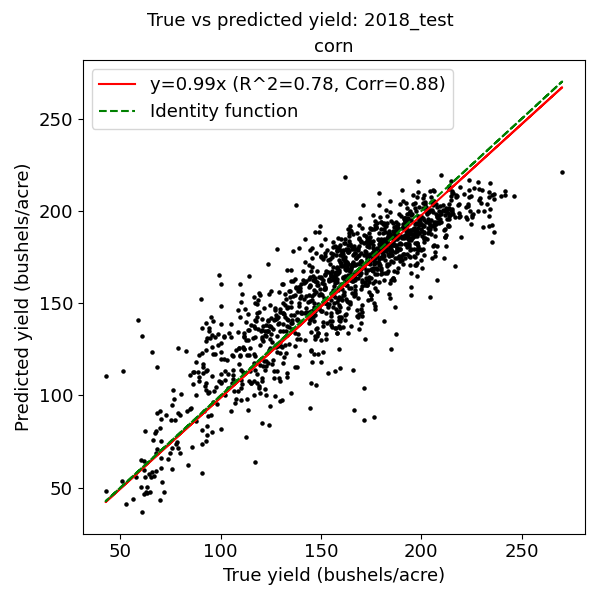
\includegraphics[width=0.8\columnwidth]{figs/true_vs_predicted_scatter_corn_2018_test.png}
\caption{Predicted vs. ground truth corn yields in 2018}
\label{scatter}
\end{figure}

\begin{figure}[tb]
\centering
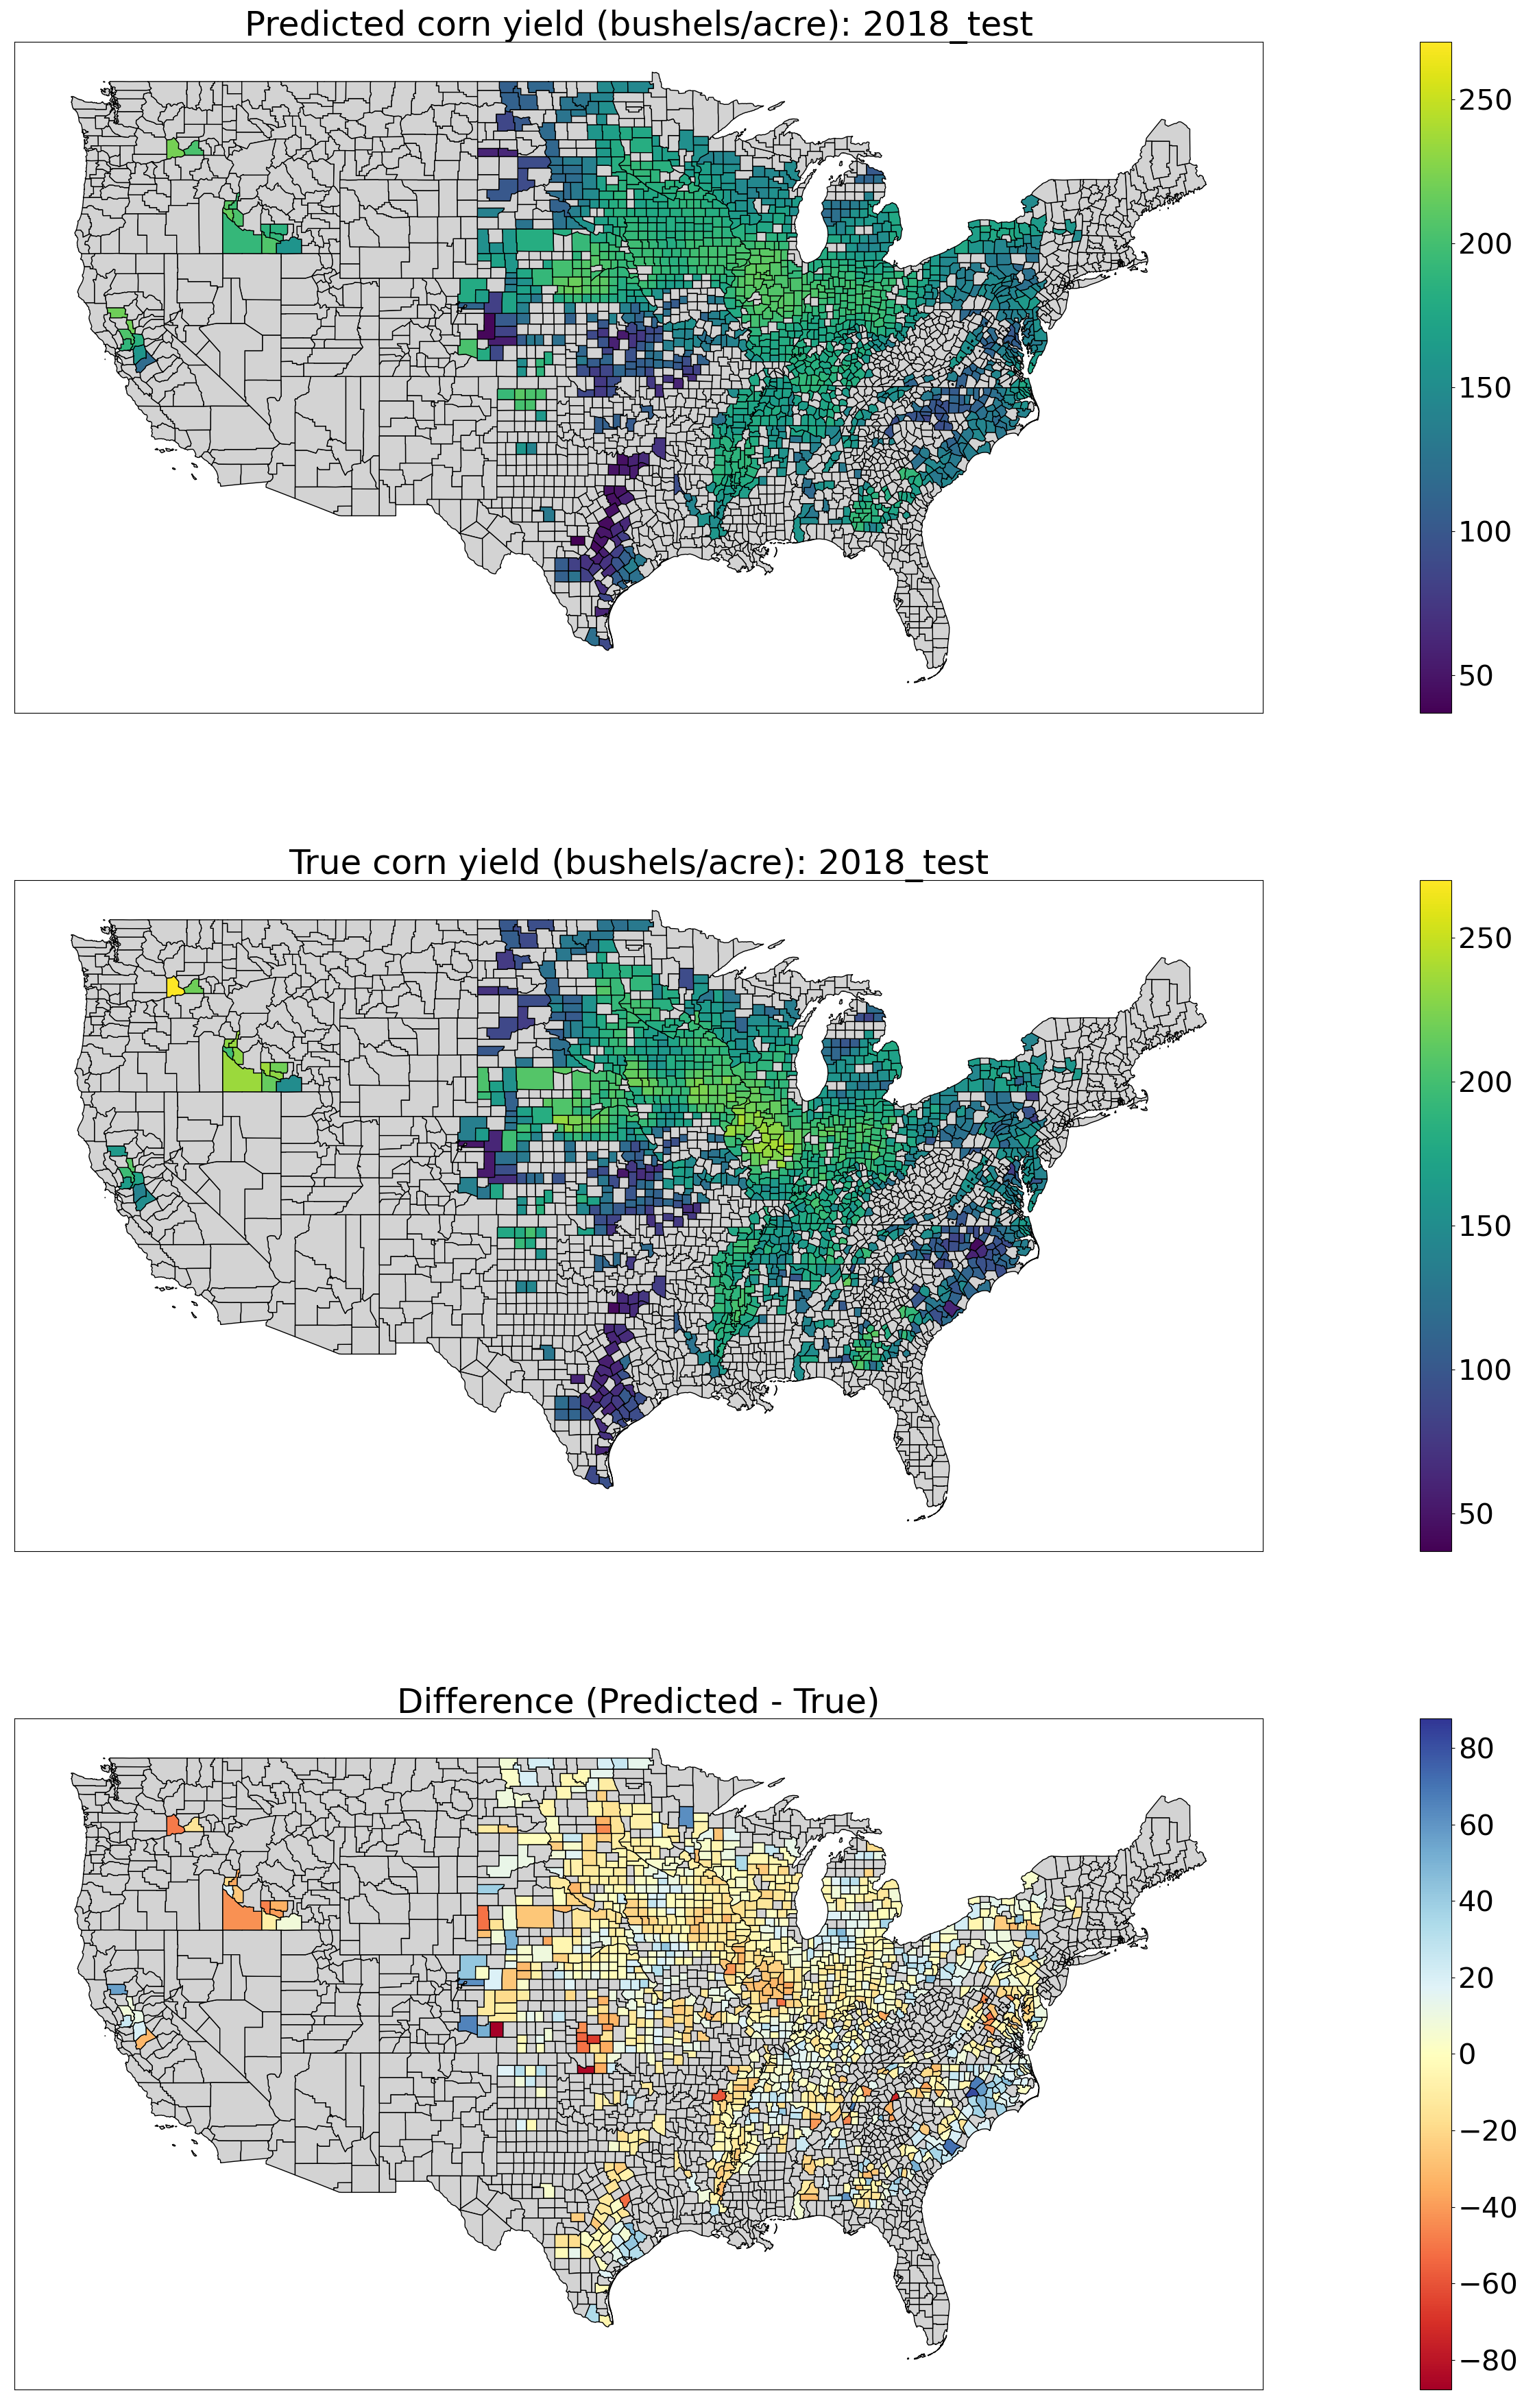
\includegraphics[width=0.95\columnwidth]{figs/true_vs_predicted_map_corn_2018_test.png}
\caption{Maps of predicted (top) and true (middle) corn yields in 2018, along with the difference (bottom). For the Difference plot, yellow means an accurate prediction, blue means the model predicted too high, and red means the model predicted too low. Gray means no data.}
\label{map}
\end{figure}

We evaluate the model on four test datasets: 2018 corn, 2018 soybean, 2019 corn, and 2019 soybean. These datasets span a wide geographic area, as well as differing growing conditions (2019 was a bad year due to the wet spring in the Midwest, which caused planting to be delayed). The results on these datasets are shown in Table \ref{results}. For the methods that only use 1 year when making predictions, our GNN model clearly outperforms comparable baselines across all datasets and metrics (except for 2018 soybean Corr, where it is slightly worse than GRU). For the methods that use a history of 5 years, our GNN-RNN outperforms competing baselines in almost all cases (except for 2018 soybean Corr, where it is slightly worse than CNN-RNN). For example, in 2019, our corn yield prediction on $R^2$ score is 16\% better than the prediction of a state-of-the-art work \cite{khaki2020cnn}. On average, we achieve a relative $R^2$ improvement of 10.44\% over the recent CNN-RNN model, 16.16\% over the 5-year LSTM, and a relative RMSE improvement of 9.6\% over the CNN-RNN model, 13.18\% over the 5-year LSTM.  These indicate the importance of exploiting geospatial context in making these predictions.




Figure \ref{scatter} shows an example scatterplot of true vs. predicted corn yields for the test year 2018. The GNN-RNN model is able to capture differences in yield between counties quite well. One minor issue is that the model is not able to capture the counties with very high yields very well; the model almost never predicts a yield higher than 220, but there are actually several counties with a true yield higher than this. This may stem from the fact that such high yields were almost never seen before in the training years. % (recall that yields tend to increase over the years). so the model is not trained to predict such high values.

We can also see these trends in the map (Figure \ref{map}). While the GNN-RNN model captures large-scale trends in crop yield very well, it sometimes outputs overly smooth predictions within a region, and under-predicts the area of high true yield in the Midwest. Improving the GNN's ability to detect fine-scale variations without smoothing them out is an important area for future work. 

We can see that crop yield prediction on a large scale is rather challenging, due to the complexity of the prediction task and the data involved. Each data point (one county/one year) has over 6,000 features, and standard models can easily overfit to noise in the data and fail to generalize. In order for the prediction task to be tractable, a model needs to take advantage of the various forms of structure in the data; temporal structure within a year (to capture weather patterns in different times of the year), temporal structure across years (to capture long-term trends such as technological improvements), and geospatial structure (to capture correlations between nearby county yields).  Our GNN-RNN model is the first model to take all of these aspects into account when making crop yield predictions, and achieves superior performance compared with the existing state-of-the-art. 

\subsection{Early Prediction}

In practice, crop yield predictions are most useful if they can be made well before harvest, as this gives time for markets to adapt, and humanitarian aid to be organized in cases of famine \cite{you2017deep}. To simulate this, at test time only, for each county we mask out all weather and land surface features from after June 1 (week 22) of the test year, and replace them with the average values for that county during the training years. Then we pass the masked features through a pre-trained model to obtain predictions. The results for several methods for 2018 corn are presented in Table \ref{early}. The graph-based models (GNN and GNN-RNN) clearly outperform competing baselines in this scenario, again illustrating the importance of utilizing geospatial context.



% \subsection{XXX}
% \junwen{qualitative results such as plots, and maybe some extra experiments depending on the space. otherwise, we put them to the supp}